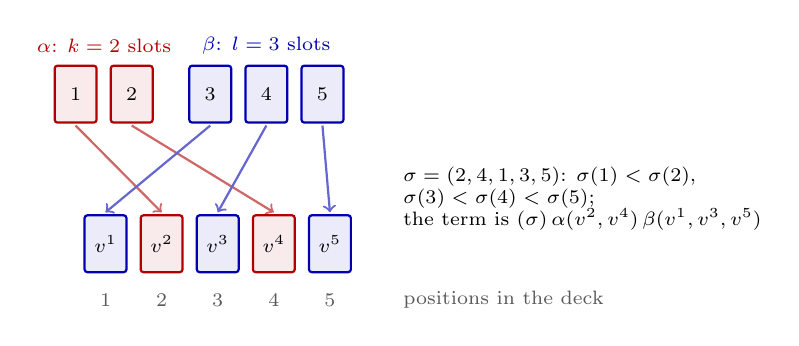
\begin{tikzpicture}[scale=0.95]
\draw[thick, red!70!black, fill=red!70!black!8, rounded corners=1pt] (0.27,1.62) rectangle (0.83,2.38); \node[font=\scriptsize] at (0.55,2.00) {$1$};
\draw[thick, red!70!black, fill=red!70!black!8, rounded corners=1pt] (1.02,1.62) rectangle (1.58,2.38); \node[font=\scriptsize] at (1.30,2.00) {$2$};
\draw[thick, blue!70!black, fill=blue!70!black!8, rounded corners=1pt] (2.07,1.62) rectangle (2.63,2.38); \node[font=\scriptsize] at (2.35,2.00) {$3$};
\draw[thick, blue!70!black, fill=blue!70!black!8, rounded corners=1pt] (2.82,1.62) rectangle (3.38,2.38); \node[font=\scriptsize] at (3.10,2.00) {$4$};
\draw[thick, blue!70!black, fill=blue!70!black!8, rounded corners=1pt] (3.57,1.62) rectangle (4.13,2.38); \node[font=\scriptsize] at (3.85,2.00) {$5$};
\node[font=\scriptsize, red!70!black] at (0.93,2.65) {$\alpha$: $k = 2$ slots};
\node[font=\scriptsize, blue!70!black] at (3.1,2.65) {$\beta$: $l = 3$ slots};
\node[font=\scriptsize, gray!70!black] at (0.95,-0.75) {$1$};
\node[font=\scriptsize, gray!70!black] at (1.70,-0.75) {$2$};
\node[font=\scriptsize, gray!70!black] at (2.45,-0.75) {$3$};
\node[font=\scriptsize, gray!70!black] at (3.20,-0.75) {$4$};
\node[font=\scriptsize, gray!70!black] at (3.95,-0.75) {$5$};
\draw[->, red!70!black!60, thick] (0.55,1.58) -- (1.70,0.42);
\draw[thick, red!70!black, fill=red!70!black!8, rounded corners=1pt] (1.42,-0.38) rectangle (1.98,0.38); \node[font=\scriptsize] at (1.70,0.00) {$v^{2}$};
\draw[->, red!70!black!60, thick] (1.30,1.58) -- (3.20,0.42);
\draw[thick, red!70!black, fill=red!70!black!8, rounded corners=1pt] (2.92,-0.38) rectangle (3.48,0.38); \node[font=\scriptsize] at (3.20,0.00) {$v^{4}$};
\draw[->, blue!70!black!60, thick] (2.35,1.58) -- (0.95,0.42);
\draw[thick, blue!70!black, fill=blue!70!black!8, rounded corners=1pt] (0.67,-0.38) rectangle (1.23,0.38); \node[font=\scriptsize] at (0.95,0.00) {$v^{1}$};
\draw[->, blue!70!black!60, thick] (3.10,1.58) -- (2.45,0.42);
\draw[thick, blue!70!black, fill=blue!70!black!8, rounded corners=1pt] (2.17,-0.38) rectangle (2.73,0.38); \node[font=\scriptsize] at (2.45,0.00) {$v^{3}$};
\draw[->, blue!70!black!60, thick] (3.85,1.58) -- (3.95,0.42);
\draw[thick, blue!70!black, fill=blue!70!black!8, rounded corners=1pt] (3.67,-0.38) rectangle (4.23,0.38); \node[font=\scriptsize] at (3.95,0.00) {$v^{5}$};
\node[font=\scriptsize, anchor=west, align=left] at (4.8,0.6) {$\sigma = (2, 4, 1, 3, 5)$: $\sigma(1) < \sigma(2)$,\\ $\sigma(3) < \sigma(4) < \sigma(5)$;\\ the term is $\sgn(\sigma)\,\alpha(v^2, v^4)\,\beta(v^1, v^3, v^5)$};
\node[font=\scriptsize, gray!70!black, anchor=west] at (4.8,-0.75) {positions in the deck};
\end{tikzpicture}
